\documentclass[a4paper]{article}

%% Language and font encodings
\usepackage[ngerman]{babel}
\usepackage[utf8x]{inputenc}
\usepackage[T1]{fontenc}

%% Sets page size and margins
\usepackage[a4paper,top=3cm,bottom=2cm,left=3cm,right=3cm,marginparwidth=1.75cm]{geometry}
%\usepackage{a4wide}
\usepackage[onehalfspacing]{setspace}

%% Useful packages
\usepackage{amsmath}
\usepackage{graphicx}
\usepackage[colorinlistoftodos]{todonotes}
\usepackage[colorlinks=true, allcolors=blue]{hyperref}
\usepackage{csquotes}
\usepackage{listings}
\usepackage{siunitx}

\title{%
  Reaktionsspiel mit Bandgeräten \\
  \large Softwareprojekt: Internetkommunikation}
\author{Steve Dierker, Patrick Hjort, Semjon Kerner}

\begin{document}
\maketitle

\section{Einführung}
\label{sec:intro}
Ziel dieses Projektes ist es, die PDP11 im Foyer des Informatikinstituts der FU Berlin zu präsentieren. Dazu verschmelzen wir es mit einem modernen Mikrocontroller und geben ihm die Kontrolle über das vorhandene Bandlaufwerk im PDP11. Mit ein paar zusätzlichen LEDs und LCD Zucker darauf sind wir in der Lage, eine einfache Gaming-Plattform für speziell entwickelte Spiele zu bauen. Ziel dieses Projektes ist es, die Hardware fertig zu stellen und ein Beispielspiel zu implementieren, bei dem zwei Spieler in der Reaktionszeit gegeneinander antreten können.

\section{Retro11}
Dies ist die C-basierte RIOT-Anwendung zur Steuerung des vorhandenen PDP11-Bandlaufwerks, einer zusätzlichen LCD-Anzeige und LEDs. Neben der Kontrolle über die vorhandene Hardware wird diese Anwendung mit einem einfachen Spiel ausgeliefert, um in der Reaktionszeit zu konkurrieren, was weiter unten erklärt wird. Um Spieler gegeneinander antreten zu lassen, ist es notwendig, zwischen den Spielplattformen zu kommunizieren. Dazu implementiert die Anwendung einen COAP-Client und -Server.

Für dieses Spiel haben Sie mindestens zwei Spieler, die beide vor einem der PDP11 an der FU Berlin stehen. Zuerst werden sie aufgefordert, dort einen Nickname einzugeben, der an den zentralen Server geschickt wird, um später die Reaktionszeit zu speichern und einen Highscore anzuzeigen. Das Spiel startet die Bandlaufwerkmotoren der beiden Knoten und sobald sie gestoppt werden, wird der Spieler aufgefordert, so schnell wie möglich zu reagieren und einen Knopf zu drücken. Die Zeit zwischen dem Anhalten des Motors und der Reaktion des Spielers ist die Reaktionszeit, die dann zur Ermittlung des Siegers herangezogen wird. Den Highscore können Sie in der Webapplikation von team2 des diesjährigen Softwareprojekts nachschlagen.

Was das Anwendungsdesign selbst betrifft, initialisieren wir zunächst alle unsere Treiber und starten dann vier Threads, um die verschiedenen Aspekte unserer Anwendung zu steuern. Der erste Thread ist der MotorController, der auf Meldungen zum Starten oder Stoppen des Motors wartet. Da wir die Motoren für eine bestimmte Zeit benötigen, kann man auch ein Timeout passieren, nach dem der Motor gestoppt werden soll. Der zweite Thread ist der CoapServer, der die Kommunikation zwischen den einzelnen Knoten handhabt und die Endergebnisse auch an das RasperryPi von team2 weiterleitet, um eine webfähige Highscore zu erstellen. Der dritte Thread ist das Spiel selbst, das die Kontrolle über alle Peripheriegeräte übernimmt und mit dem CoapServer über eine Shared-State-Variable kommuniziert. Das Spiel steuert die Benutzereingaben und -ausgaben und bietet ein Arcade-ähnliches Spielerlebnis. Der vierte und letzte Thread dient zu Debugging-Zwecken und führt einfach eine Shell mit benutzerdefinierten Befehlen für Hardware-Diagnose und andere Debuggingoperationen aus. Er ist nur zugänglich, wenn ein Computer an den USB-Port des SAMR21 Xpro angeschlossen wird.

\section{Hardware}
\label{sec:hw}
\subsection{vorhadene HW}
Ein paar einleitende Sätze
\begin{enumerate}
	\item samr21 Xpro
	\item Multiplexer S74LS151 und Buttons
    \item LED Stripe WS2811 und WS2812B
    \item LCD DOGL128B-6
    \item L298H-Modul
	\item ATX Netzteil
	\begin{enumerate}
		\item Spannungen
	\end{enumerate}
\end{enumerate}
Retro11 ist eine C-basierte RIOT-Anwendung, die auf dem Mikrocontroller SAMR21 XPro läuft. Zunächst haben wir mit der Entwicklung der Hardwareplattform und dem Schreiben von Treibern für jedes Peripheriegerät begonnen, da diese noch nicht von RIOT selbst unterstützt wurden. Jeder Treiber ist entsprechend den von RIOT angebotenen Beispieltreibern implementiert. Die Treiberimplementierung war für alle Peripheriegeräte außer dem WS2811 unkompliziert. Der WS2811 bietet einen digitalen Eingang zum Empfang von Farbinformationen und einen digitalen Ausgang zum Senden von Farbinformationen an den nächsten WS2811 in Reihe. Zum Schluss steuert jede WS2811 eine LED und bis zu 1024 WS2811 können miteinander verkettet werden, um ganze LED-Arrays zu steuern. Da der WS2811 nur ein Einleiter-Protokoll und keine zusätzliche Taktung anbietet, benötigt er für die Unterscheidung zwischen 0 und 1 in seinem Protokoll harte Timings. Für unser Projekt haben wir zwei verschiedene WS2811 LED-Sets gekauft. Das erste ist ein bereits montierter LED-Streifen, der mit unserem Treiber aus der Box heraus gearbeitet hat und das zweite ist ein Set von separaten Chips und LEDs, die Sie selbst zusammenbauen können. Der zweite Kit weigerte sich, mit unserem Treiber zu arbeiten und nach mehrtägigen Debugging-Tests stellte sich heraus, dass der Controller eine gemeinsame Annode benötigt, aber die LEDs, die wir erhielten, boten eine gemeinsame Kathode. Leider war der Shop, bei dem wir die LEDs gekauft haben, nicht in der Lage, die richtigen LEDs rechtzeitig zur Verfügung zu stellen, um das Projekt komplett abzuschließen.
\subsection{zusätzliche HW}
\subsection{Treiber}

\section{Netzwerkkommunikation}
\label{sec:net}
Die Kommunikation zwischen den Plattformen erfolgt über das RESTful Constrained Application Protocol, CoAP, das Nachrichten über UDP und IPv6 sendet, wie in Abbildung \ref{fig:seq_diagram} . Ein Mikrocontroller führt eine Client-Applictation aus, die das Spiel steuert. Die benötigten Informationen werden von einer Server-Anwendung bereitgestellt, die auf jedem Mikrocontroller ausgeführt wird. Abhängig vom Spielstatus fragt der Client die Ressource mit den erforderlichen Informationen beider Server mit einer Get-Methode ab, bis die Server die Informationen bereitstellen, um zur nächsten Stufe überzugehen. Im ersten Zustand fordert der Client die Nicknamen des Spielers an, fordert dann das eigentliche Reaktionsspiel auf, im zweiten Zustand zu starten, fordert die Reaktionszeit im dritten Zustand an und fordert jede Maschine auf, sich anzeigen zu lassen, ob sie im letzten Zustand gewonnen oder verloren hat. Zusätzlich verfügen beide Server über eine Ressource, die auf Wunsch von team2 Highscore-Informationen im SenML-Format bereitstellt.
\begin{figure}[h]
\centering
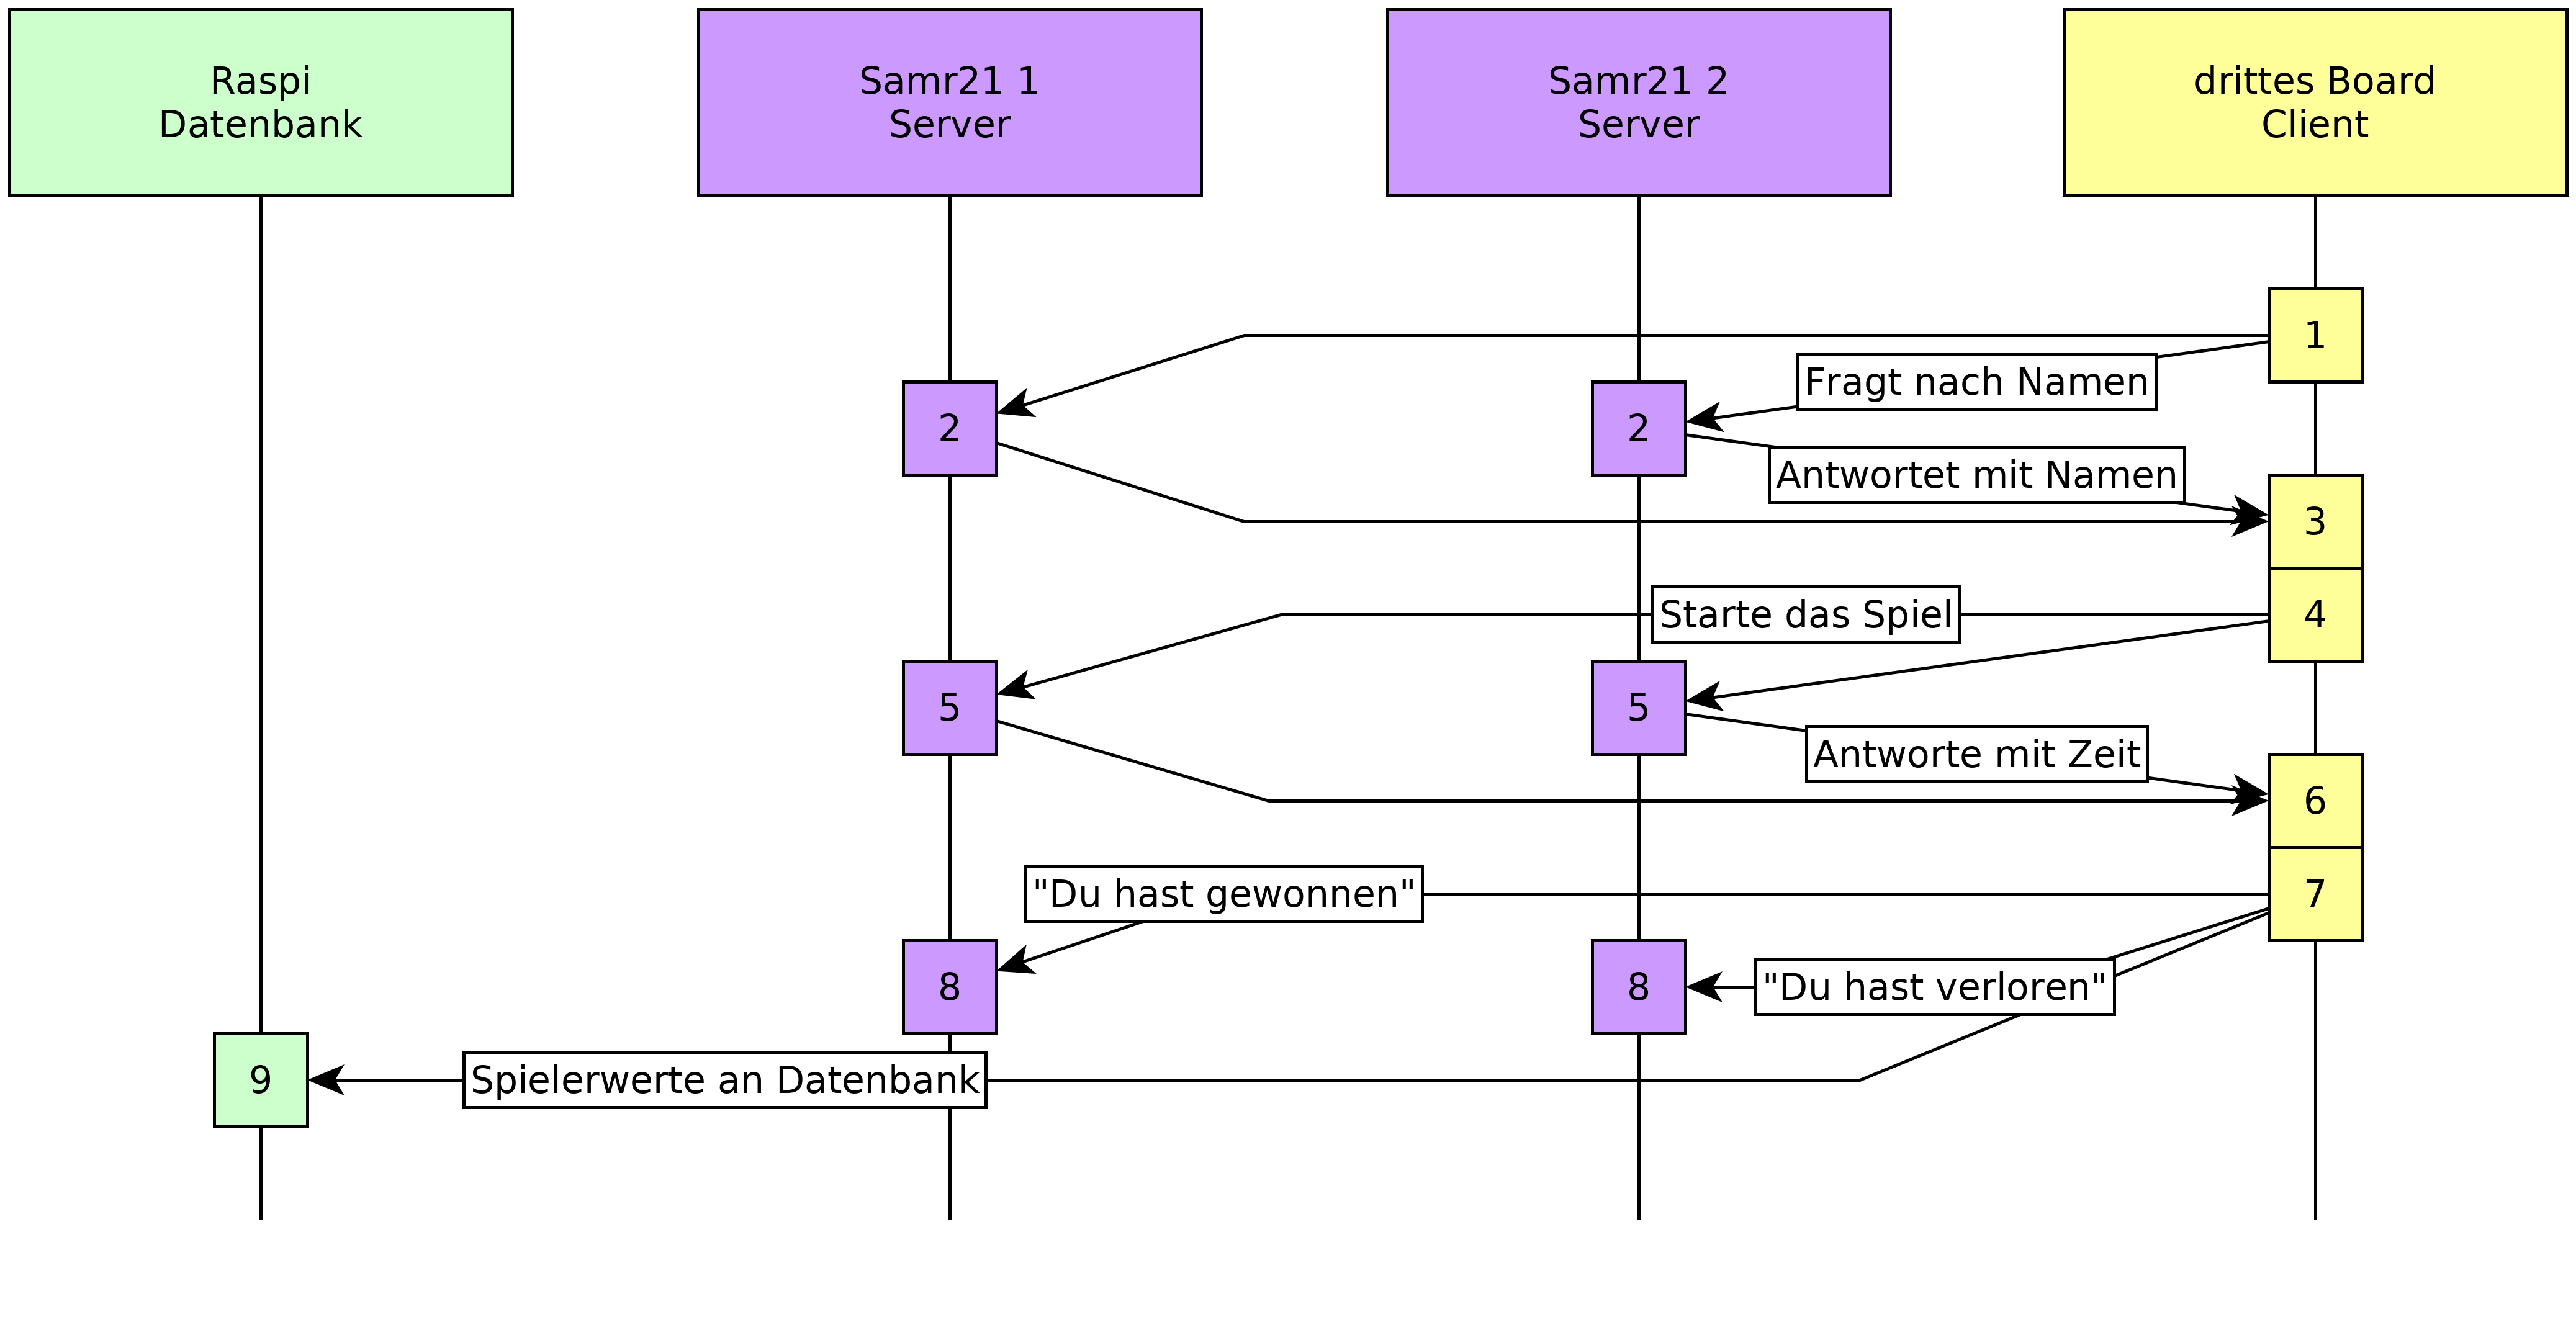
\includegraphics[scale=0.1]{team1_kommunikation.png}
\caption{\label{fig:seq_diagram}Sequenzdiagramm der Anwendung}
\end{figure}

\section{Stand der Umsetzung}
\label{sec:status}
\subsection{Stand}
Kommunikation zwischen Knoten
Hardware $(H-brücke, Motor, Multiplexer, Buttons, LCD, LED-Stripe )$
Treiber
Basisspiel
\subsection{Probleme}
LEDs von Buttons fehlen
Kommunikation mit Raspi/Website/Coap-Gateway
LCD Kontrast
LCD Backlight
\subsection{Rückblick auf Zeitplan}
Zeitplan nicht eingehalten
Hardware hat mehr Zeit gekostet als erwartet
Probleme mit Netzwerkkommunikation
Gar nicht nach Magnetbändern gesucht
Spiel runterschreiben ging am Ende dann schnell
Entwurf Poster war schnell aber nicht so früh wie geplant

\section{Weiterführende Arbeit}
\label{sec:further}
Da die LEDs für die Buttons leider nicht eingebaut werden konnten ist eine sinnvolle Weiterführung des Projekts die LEDs zu ergänzen und Funktionen zu entwickeln, so dass die aktuell drückbaren Buttons auch entsprechend ihres Zweckes farbig aufleuchten. So kann eine Menüführung deutlich offensichtlicher abgebildet werden, als es derzeit der Fall ist, da bisher die Spieler nicht erkennen können, welche Buttons welchem Zweck dienen.
Weiterhin war es geplant Ersatz für die fehlenden Button-Aufsätze mittels 3D-Druck auszudrucken. Entsprechende Modelle sind bereits im Repository enthalten.
Da stets nur ein einzelner Button im Interruptmodus betrieben werden kann und mehrere Buttons gepollt werden müssen entstehen Latenzen bei der Eingabe durch den Nutzer. Es ist möglich, dass hier eine Designänderung eine bessere Nutzererfahrung schafft.
Die Motoren müssen gereinigt werden.
Eine weitere Möglichkeit der Erweiterung des Projekts wäre das hinzufügen von weiteren Spielen. Ein denkbarer Ansatz ist es eine LUA-API zu entwerfen, so dass neue Spiele abstrahiert bzw. hochsprachig geschrieben werden können und so schnell eine Vielzahl von Spielen für die Hardware zur Verfügung gestellt werden kann. So kann vorraussichtlich die Häufigkeit der Nutzung gesteigert, aber auch die Akzeptanz durch die Studenten gesteigert werden, welche ihre eigenen Spiele schneller und nur mit wenige Aufwand auf der Hardware ausprobieren können.
Eine optimale Lösung um neu hinzugefügte Spiele auf den Boards auszuführen wäre das Ausführen regelmäßiger over-the-air-updates welche die redegierten Spiele aus den entsprechenden Paketquellen auf die Boards flashen.

\end{document}
